%  !TEX root = ../main.tex
~
% \vfill\eject
\section*{Appendix}
\setcounter{equation}{0}
\setcounter{subsection}{0}
\setcounter{section}{0}
\renewcommand{\theequation}{\arabic{equation}}
\renewcommand{\thesubsection}{\arabic{subsection}}
\renewcommand{\thesection}{\Alph{section}}

\section{Single-sideband Amplitude Modulation}\label{append:SSB}
In this section, we give mathematical proof that the baseband perturbation of SSB-AM signals can be recovered by commercial microphones. We initially compare the maximum energy of USB-AM and LSB-AM emitting the same perturbation when sound leakage occurs, and LSB-AM is 87\% of USB-AM. Thus, we adopt the USB-AM in our attacks due to its better inaudibility:
\begin{equation*}
\begin{aligned}
    & \text{USB-AM:}~ S_{USB}(t)=m{cos\omega_{c}t}-\hat{m}{sin\omega_{c}t}+cos\omega_{c}t\\
    & \text{LSB-AM:}~ S_{LSB}(t)=m{cos\omega_{c}t}+\hat{m}{sin\omega_{c}t}+cos\omega_{c}t
\end{aligned}
\label{equ:SSB_formula}
\end{equation*}
where the $\hat{m}$ is the conjugate of $m$. The microphone amplifier's output is below:
$$S_{out} = k_{1}S_{USB}(t) + k_{2}S_{USB}^2(t) + \cdots$$
The $S_{USB}^2(t)$ term has three components: a high-frequency $2\omega_{c}t$ components:
$$(m+1) \hat{m} \sin(2 \omega_c t)+\frac{m^2+2m+1-\hat{m}^2}{2} \cos(2\omega_c t)$$
a direct current (DC) term $\frac{1}{2}$ and an audible component $S_{aud}(t)=\frac{1}{2}(m^2+2m+\hat{m}^2)$.
$S_{USB}(t)$ and the high-frequency component are filtered by the low-pass filter because its frequency is above 25~kHz. The DC component is filtered by the microphone’s capacitor. Thus, the audible component $S_{aud}(t)$ that passes the microphone filtering system can function to ASR.
\vfill\eject

\section{Real-world Scenario}\label{append:attack_scenario}
Figure~\ref{fig:attack_actual} presents our real-world attack scenario.
\begin{figure}[h]
	\centering
	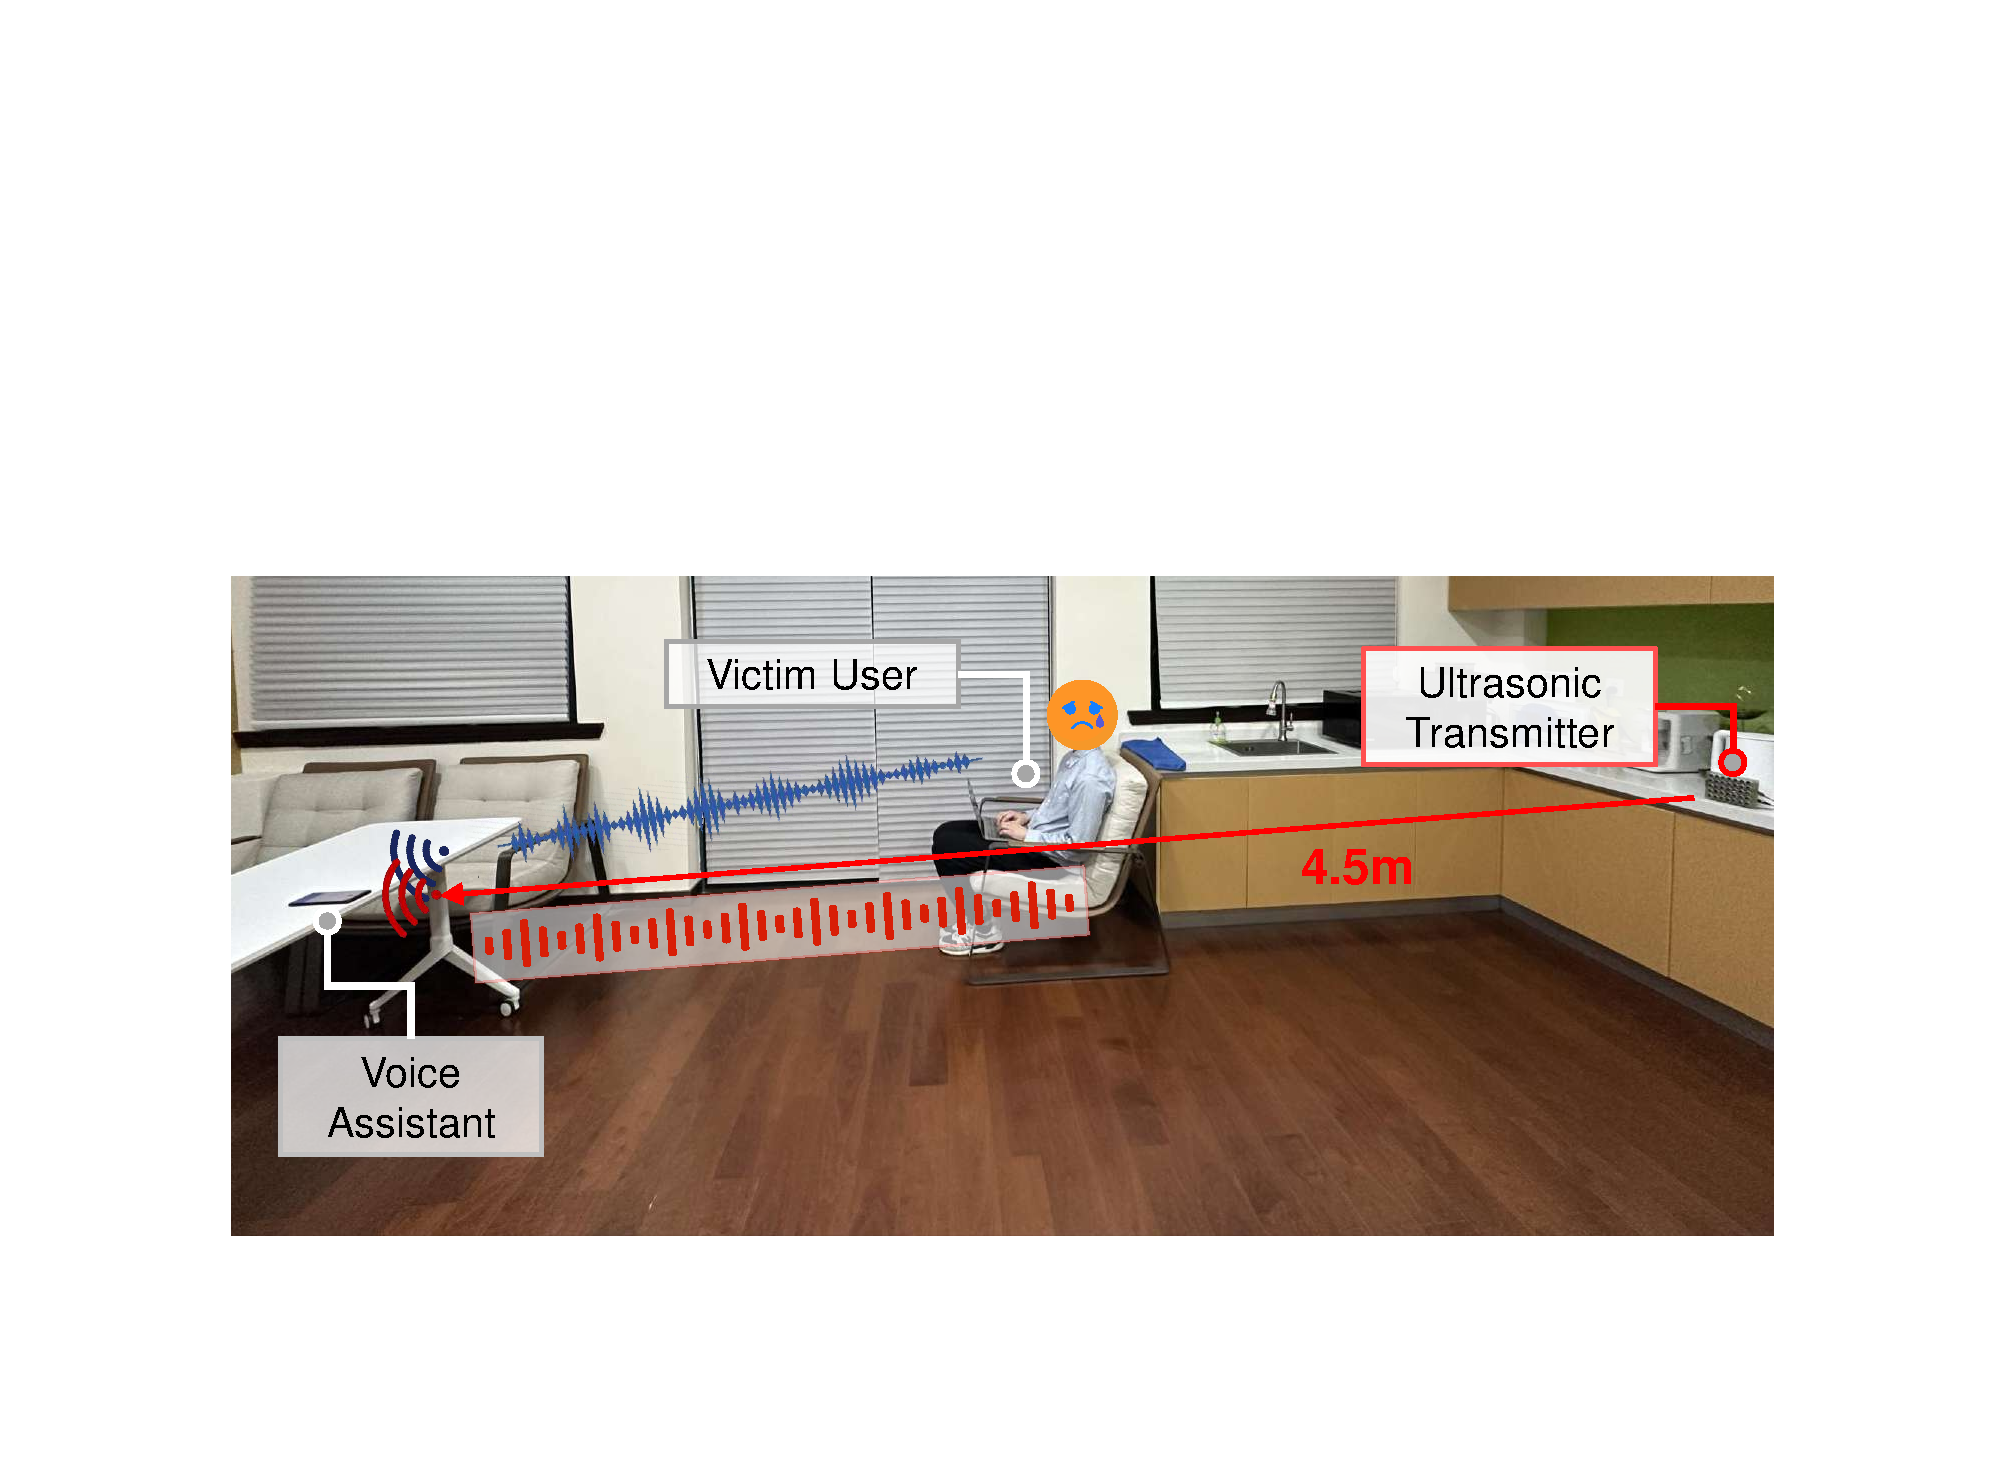
\includegraphics[width=0.48\textwidth]{exp_setup_actual2.pdf}
	\caption{\label{fig:attack_actual}Real-World Attack Scenario.}
	% \vspace{-10pt}
\end{figure}


\section{Algorithm of \alias}\label{append:algo1}
Given that technical workflow for the silence and universal perturbation are overall identical, the major differences are the optimization objective: $y_t/y_b$ and hyper-parameters. Therefore, we demonstrate \alias's representative optimization process of crafting a universal perturbation from scratch in Algorithm.~\ref{algo1}.
% \vfill\eject

\begin{algorithm}[h]
	\caption{Universal \alias Generation}
	\label{algo1}
	\LinesNumbered
	\KwIn{The ASR model with CTC Loss Computation module: $\mathcal{L}$, the maximum epoch: $\text{maxEpoch}$, the desired loss: $objValue$, with a scoring module: $S$, the learning rate: $\eta$, the preset time range: $T$.}
	\KwOut{The universal perturbation $\delta$}
	\textbf{Init} $\delta \gets 0^N$\\
	\For{$1$ to ${ maxEpoch}$}
	{
		${J} \gets 0$\\
            \For{$h_{\theta}\in U_H$, $n\in U_N$}
            {
                $\hat{e} = e^{-a_0 \omega_{c}^{n}d}$\\
                $\overline{\delta} = h_{\theta}\hat{e}\ast \overline{\delta:\hat{\xi}} + n$\\
                \For{$x\in U_x, g\in G, S_{(\cdot)}~{s.t.}~T$}
                {
                    $\Tilde{x}=\beta\cdot g\ast x$\\
                    $\Tilde{x_{\delta}} = clip(\Tilde{x}+\mathcal{S}_{(\overline{\delta})}, [-1,1])$\\
                    $J+=\mathcal{L}(\Tilde{x_{\delta}}, y_t)$
                }
            }
            Compute ${\nabla}_\mathcal{\delta}J$\\
            $\delta \gets \Omega_{Adam}(\delta+\eta\cdot {\nabla}_\mathcal{\delta}J )$\\
            $\delta \gets clip(\delta, [-1,1])$\\
            \If{$J \le objValue$}{break}
        }
	% return $\text{\alias}(\mathcal{A,K})$
	\normalsize
\end{algorithm}
\vfill\eject

\section{Targeted Commands Lists}\label{append:command_list}
Tab.\ref{tab:diff_commands} lists 10 different commands, corresponding to the performance of constructing target command-specific perturbations in experiment \textsection\ref{sec:eval_commands}.
\begin{table}[h]
	\centering
        \normalsize
		\caption{Attack with Different Targeted Commands}
		\renewcommand\arraystretch{0.9}
		\renewcommand\tabcolsep{1.5pt}
		\begin{threeparttable}
			\begin{tabular}{l|c|c}
                \toprule
                \textbf{Target Command} & \textbf{~~~~SR~~~~} & \textbf{~~CER~~} \\
				\midrule
                    ``Start recording''  & 100\% & 0\% \\ \midrule
				``Set a timer''  & 100\%  & 0\% \\ \midrule
				``Open the door''  & 100\% & 0\% \\ \midrule
				``Take the picture''  & 100\% & 0\% \\ \midrule
				``Call nine one one (911)''  & 100\% & 0\% \\ \midrule
				``Cancel my morning alarm''  & 100\% & 0\% \\ \midrule
                    ``Turn on airplane mode'' & 94.39\% & 0.28\% \\ \midrule
                    ``Open my photo album''  & 95.03\% & 0.50\% \\ \midrule
				``What is going on Twitter?''  & 100\% & 0\% \\ \midrule
                    ``Mute volume and turn off the WiFi'' & 92.82\% & 0.21\% \\
				\bottomrule
			\end{tabular}
		% \vspace{-10pt}
		\end{threeparttable}
		\label{tab:diff_commands}
\end{table}
% \vfill\eject


\section{Different Attack Angles}\label{append:eval_angles}
In this experiment, we keep the recording device's bottom microphone spatially within the ultrasound beam's coverage and set the attack distance to 2.5m. We rotate the recording device from 0\degree to 180\degree at 15\degree intervals, among which 90\degree means the ultrasound directly points to the bottom microphone. Under each angle, we play 40 benign commands and emit the universal IAP.
Eventually, we collected 520 mixed audio signals from 13 angles. As shown in Fig.~\ref{fig:attack_angle}, although ultrasound is highly directional, we find that there is no significant difference with 100\% success rate among different angles within 15\degree$\sim$150\degree. As the deployed location of bottom microphones varies with different phones, therefore attack performance is not symmetrical with angles (i.e., 79\% at 0\degree and 49\% at 180\degree). Overall, as most voice-interface devices nowadays are equipped with omnidirectional microphones, \alias can be effective as long as the beam can cover the bottom microphone. 
\begin{figure}[h]
    \centering
    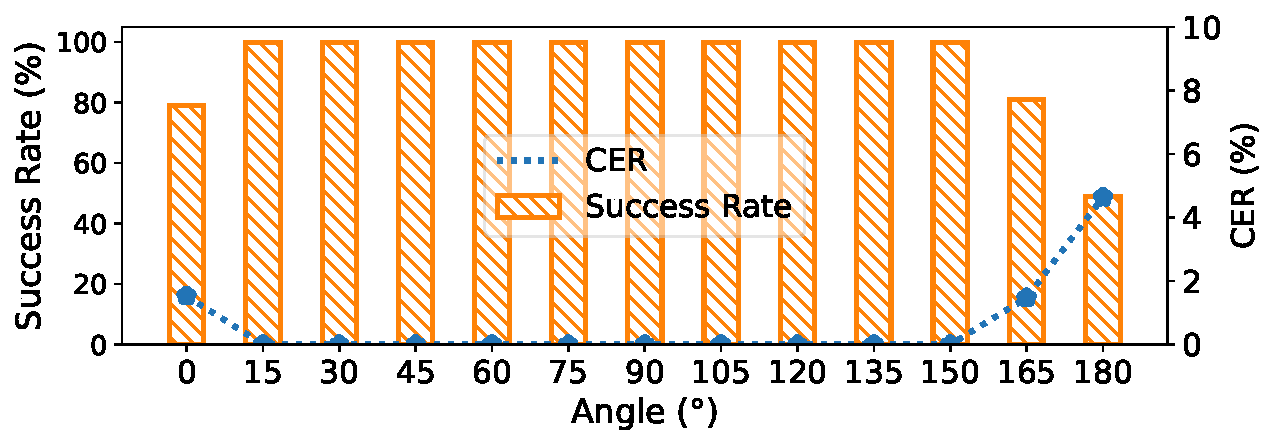
\includegraphics[width=0.45\textwidth]{attack_angle.pdf}
    % \vspace{-10pt}
    \caption{\alias's performance at different angles.}
    \label{fig:attack_angle}
\end{figure}

% \vfill\eject

\section{Different Speech \& Perturbation Loudness}\label{append:loudness_compare}
Fig.~\ref{fig:loudness_compare} shows the success rate and CER of our experiments on the relative energies between the attack perturbation and speech.
\begin{figure}[h]
	% \vspace{-7pt}
	\centering  %居中
		\subfigure[Success Rate (\%)]{   %第一张子图
		\begin{minipage}[t]{0.22\textwidth}
			\centering
                % \hspace{-0.25\linewidth}
			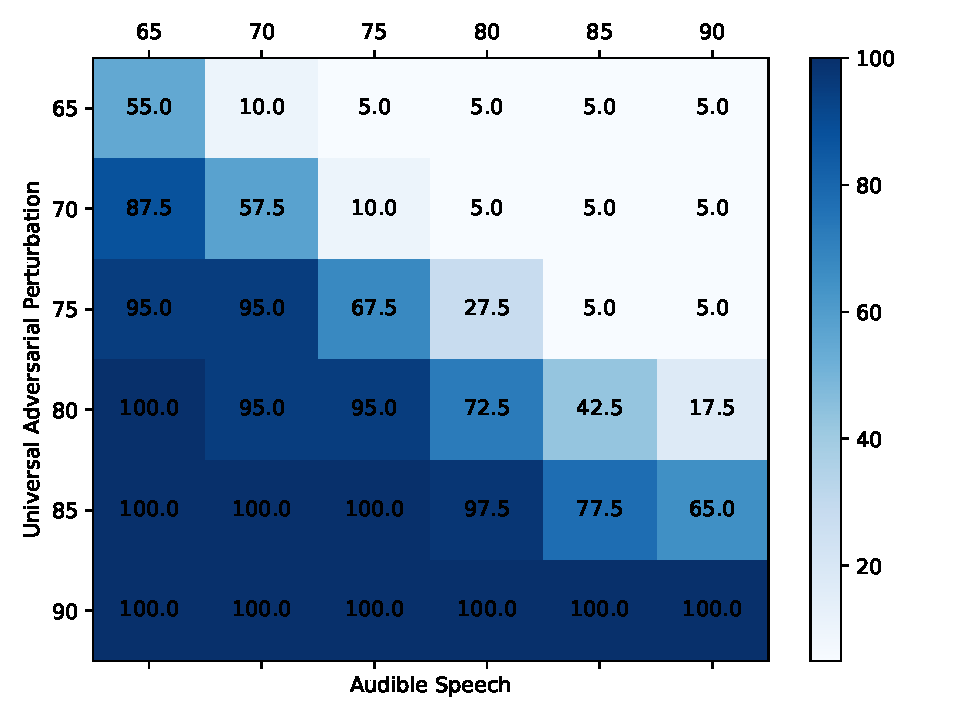
\includegraphics[width=1.1\textwidth]{snr_SR.pdf} % height=0.765\linewidth
		\end{minipage}
		}
	\subfigure[CER (\%)]{   %第一张子图
	\begin{minipage}[t]{0.22\textwidth}
		\centering
            % \hspace{-0.25\linewidth}
		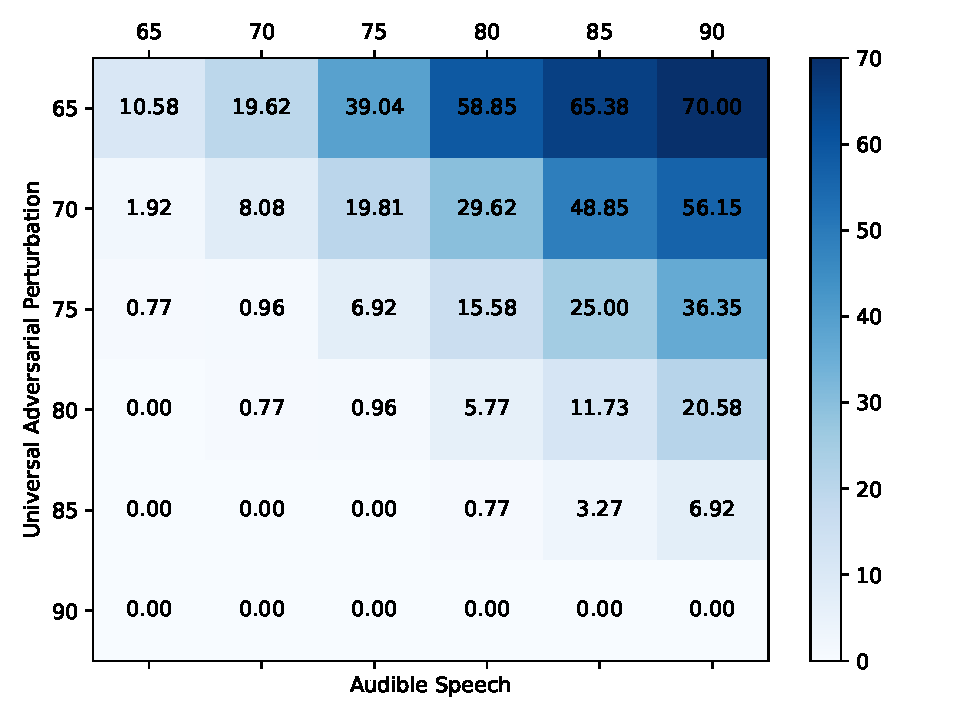
\includegraphics[width=1.1\textwidth]{snr_CER.pdf} 
	\end{minipage}
	}
	% \vspace{-10pt}
	\caption{The performance of loudness relationship between user speech and perturbation.}    %大图名称
	\label{fig:loudness_compare}    %图片引用标记
	% \vspace{-5pt}
\end{figure}
% \vfill\eject

\section{User Testing}\label{append:user_test}
In this section, we elaborate on the \textit{Man-in-the-middle} attack strategy, whose effect is akin to experiencing network congestion when users use the ASR service, resulting in slower responses. Prolonged latency can make users feel uncomfortable while using the service. 
To assess user awareness under such delays, we design 10 scenarios, each consisting of an audio clip that simulates a user issuing a command to the ASR system with random delays (1-5 seconds) before the voice assistant executes the command. 
We collected test results from 140 college students of different majors. As shown in Figure~\ref{fig:user_latency}, when the delay time is less than 2.7 seconds (the junction point of two distribution curves), more users find the ASR service comforting than uncomfortable. 
The participants are also asked to fill in what they think the cause is if they experience an uncomfortable delay when using the ASR service.
Only 11 out of 140 participants suspect an attack, while almost all others attribute the delay to network latency/congestion or device stuck, suggesting that this strategy poses a hidden attack.
We believe that users' suspicion may also be related to their disciplinary background, e.g., users with knowledge of cybersecurity are more likely to consider the possibility of an attack.

\begin{figure}[h]
    \centering
    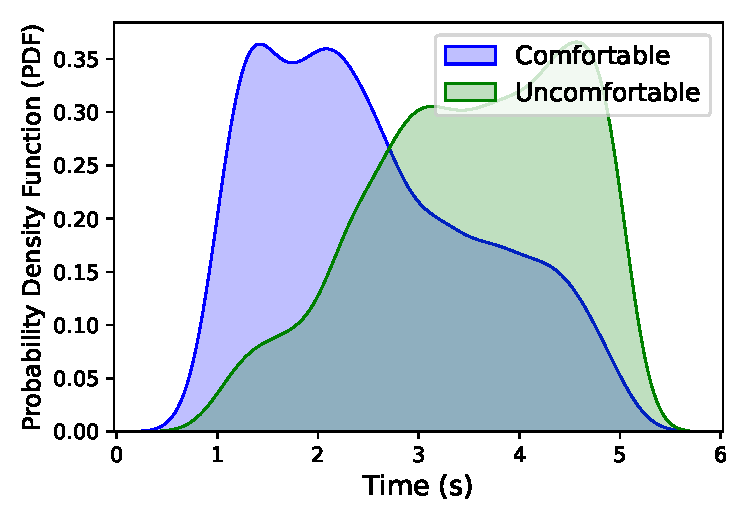
\includegraphics[width=0.45\textwidth]{latency.pdf}
    \caption{The probability distribution of users' awareness during a \textit{man-in-the-middle} attack under different delay conditions (similar to network latency). ``Comfortable'': the situation where users find the ASR service is normal and are not aware of the attack; ``Uncomfortable'': the delay may cause them to feel uncomfortable or unusual.}
    \label{fig:user_latency}
\end{figure}

